\section{Introduction}
\label{sec:intro}
% Language models (LMs) have become helpful assistants for software development~\citep{austin2021program,chen2021evaluating,li2022competition}, with programmers playing the role of intermediary between the LM and computer to successfully complete programming tasks.
% For instance, after executing LM-generated code, a programmer may request refinements from the LM based on computer feedback such as error messages.
% More recently, LMs are being used as autonomous \textit{agents} that interact with computer environments without human intervention~\citep{yang2023intercode, wu2024oscopilot, xie2024osworld}.
% This approach has the potential to accelerate software development but remains largely unexplored in realistic settings.

% Language models (LMs) have become helpful assistants for software development~\citep{austin2021program,chen2021evaluating,li2022competition}, with programmers playing the role of intermediary between the LM and computer to successfully complete programming tasks.
% For instance, after executing LM-generated code, a programmer may request refinements from the LM based on computer feedback such as error messages.
% More recently, LMs are being used as autonomous \textit{agents} that interact with computer environments without human intervention~\citep{yang2023intercode, wu2024oscopilot, xie2024osworld}.
% Are LM agents sensitive to interface design for solving programming tasks?

% Language model (LM) agents have recently emerged as a new inference mode for autonomously solving tasks within some environment.

% Recent advancements in language models have brought their capabilities to the point where they can start to interact with real-world environments to solve tasks autonomously.
% In the past, language models were primarily capable for sequence generation, but further refinements of their abilities and techniques such as react etc have extended them to 

% Generally capable LMs were first developed in a sequence generation paradigm~\cite{Radford2018ImprovingLU,radford2019language,t5}, but recent advancements in their knowledge~\cite{Brown2020LanguageMA}, reasoning~\cite{Nye2021ShowYW,Wei2022ChainOT}, and interaction techniques~\cite{yao2023react,Ouyang2022TrainingLM}, have brought them to a level such that they can start to interact with real-world environments to perform various tasks.

% Recent advancements in language models (LMs) have significantly enhanced their autonomous interaction abilities with real-world environments, evolving from prediction with simple sequence generation~\cite{Radford2018ImprovingLU,radford2019language,t5} to performing complex tasks due to improvements in knowledge~\cite{Brown2020LanguageMA}, reasoning abilities~\cite{Nye2021ShowYW,Wei2022ChainOT}, and interaction techniques~\cite{yao2023react, Ouyang2022TrainingLM}.

% Recent advancements in language models (LMs) have markedly improved their capacity for autonomous interaction with real-world environments.
% These models have evolved from a simple sequence generation paradigm~\citep{Radford2018ImprovingLU,radford2019language,t5} to acting in digital environments autonomously~\citep{Park2023GenerativeAgents, yao2023react}, thanks to advancements in knowledge\alex{wtf is knowledge and why do we cite GPT-3?}~\citep{Brown2020LanguageMA}, reasoning abilities~\citep{Nye2021ShowYW,Wei2022ChainOT}, and interaction techniques~\citep{yao2023react, Ouyang2022TrainingLM} \alex{what are interaction techniques, I'm so confused}.

Recent work has demonstrated the efficacy of LM agents for code generation with execution feedback~\citep{shinn2023reflexion}.
However, applying agents to more complex code tasks like software engineering remains unexplored.
To solve programming tasks, LM agents are typically designed to use existing applications, such as the Linux shell or Python interpreter~\citep{wu2024oscopilot, xie2024osworld,yang2023intercode}.
However, to perform more complex programming tasks such as software engineering~\citep{jimenez2024swebench}, human engineers benefit from sophisticated applications like VSCode with powerful tools and extensions.
Inspired by human-computer interaction (HCI) studies on the efficacy of user interfaces for humans~\citep{cooperaboutface}, we investigate whether LM agents could similarly benefit from better-designed interfaces for performing software engineering tasks.

\begin{figure}[ht]
\centering
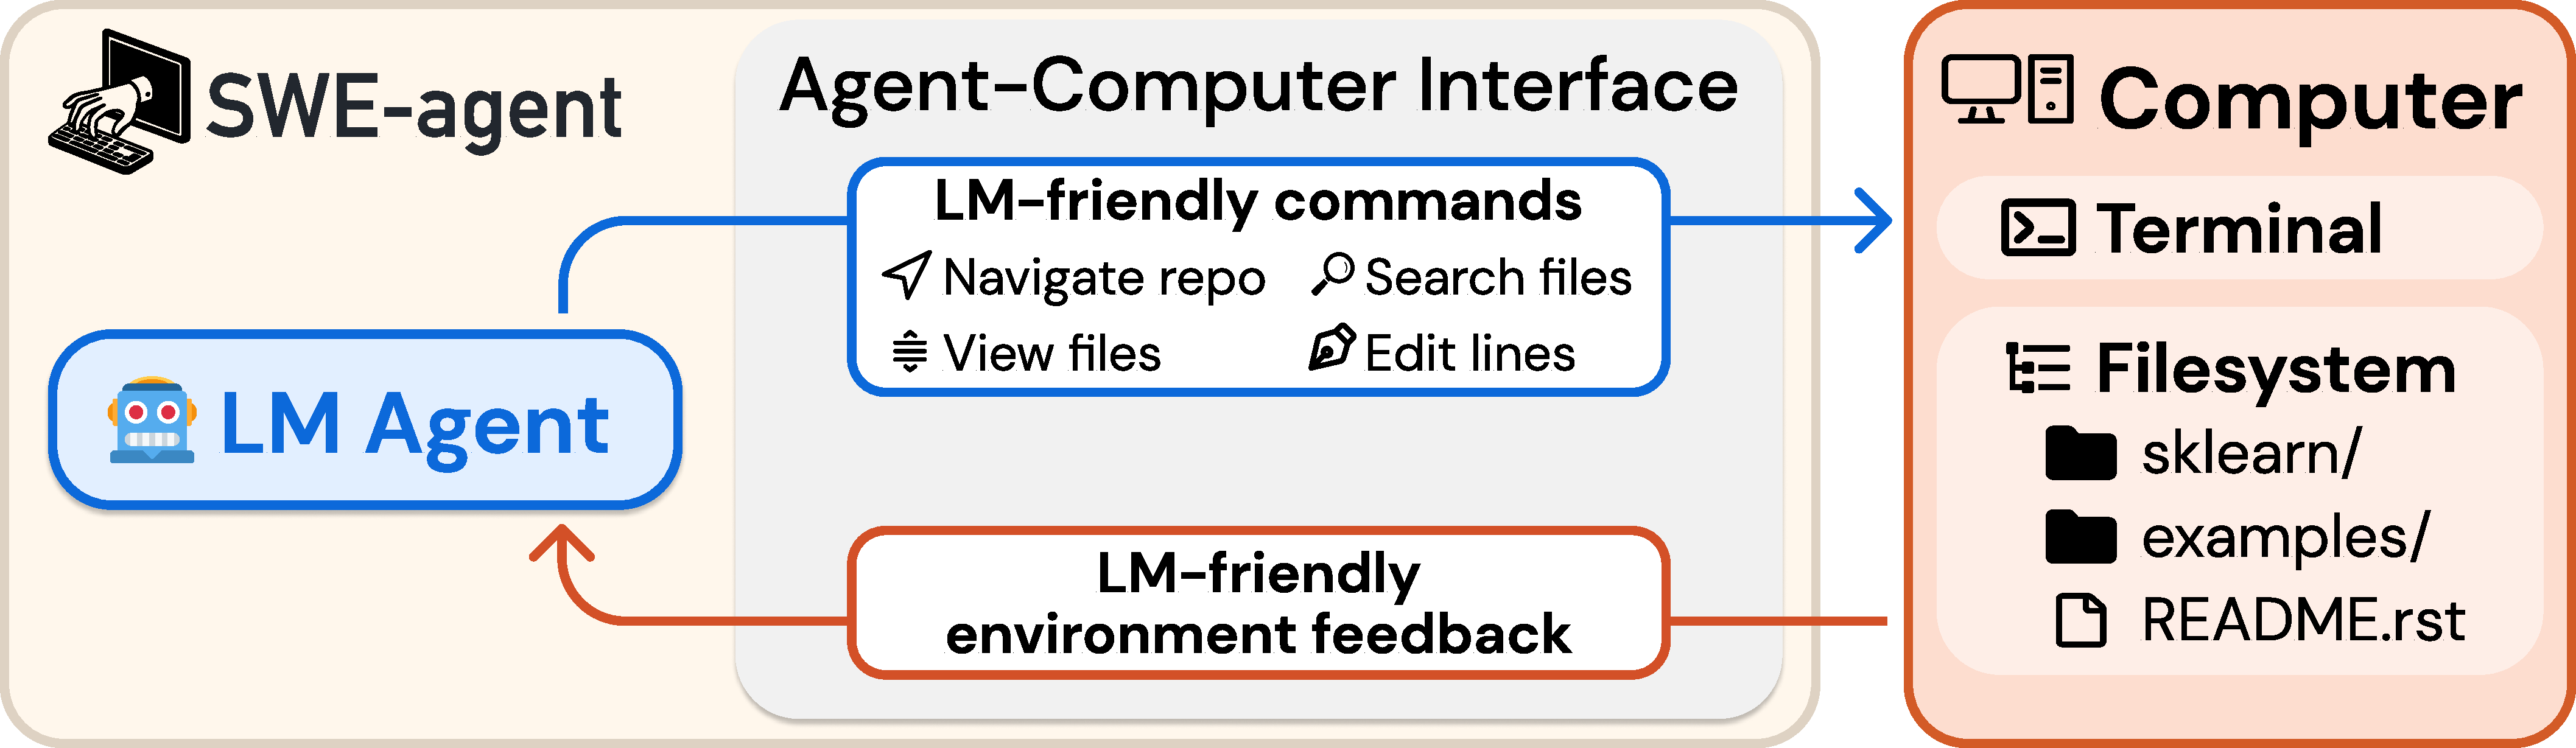
\includegraphics[width=0.67\linewidth]{figures/swe_agent_overview.pdf}
\caption{
    SWE-agent is an LM interacting with a computer through an agent-computer interface (ACI), which includes the commands the agent uses and the format of the feedback from the computer.
}
\label{fig:teaser}
\end{figure}

% \alex{This is more of a related work section than an easy invitation to a v cool paper.}
% \ofir{hmmm, this reads pretty well to me}

% In command-line environments LM agents operate within a Linux shell, utilizing common shell commands to solve programming tasks~\citep{yang2023intercode, wu2024oscopilot, xie2024osworld}.

% To support more complex programming tasks, such as software engineering~\citep{jimenez2024swebench}, human engineers benefit from sophisticated applications like VSCode with powerful tools and extensions.
% Inspired by human-computer interaction (HCI) studies on the efficacy of user interfaces for human users, we investigate whether LM agents could similarly benefit from better-designed interfaces for performing software engineering tasks.

% As our main contribution, we demonstrate the importance of designing an agent-computer interface (ACI), i.e., an abstraction layer between the LM agent and computer, to enhance the LM agent's performance (Figure~\ref{fig:teaser}).
% \textit{We find that custom ACIs tailored to LMs outperform existing user interfaces} (UIs) \textit{designed for human users}, such as the Linux shell.
% From this effort, we introduce SWE-agent, an LM-based autonomous system that interacts with a computer to solve challenging real-world software engineering problems, such as those proposed in SWE-bench~\citep{jimenez2024swebench}.

% Consider the simple setting of using a Linux shell interface~\citep{yang2023intercode} which naturally lends itself to turn-based interaction with an LM agent due to its text-only input commands and outputs.
% In practice, we find that this can be an unsuitable environment for LM agents.
% For example, it fails to provide simple commands to edit a small file segment, and does not provide any feedback if the user makes an invalid edit.
% These deficits substantially hamper performance, as we show in our results, and motivate our construction of a novel ACI for SWE-agent.

Consider the simple setting of an agent interacting directly with a Linux shell~\citep{yang2023intercode}.
In practice, we find that LM agents can struggle to reliably take actions in this environment.
For example, it fails to provide simple commands to edit a small file segment, and does not provide any feedback if the user makes an invalid edit.
These deficits substantially hamper performance, motivating the need for an agent-computer interface (ACI), i.e., an abstraction layer between the LM agent and computer, to enhance the LM agent's abilities in computer environments (Figure~\ref{fig:teaser}).

From this effort, we introduce SWE-agent, an agent composed of an LM and ACI, that can interact with a computer to solve challenging real-world software engineering problems, such as those proposed in SWE-bench~\citep{jimenez2024swebench}.
% SWE-agent's ACI provides commands for viewing, searching through and editing files. 
% It also provides specific and concise environment feedback, including informative error messages for edits that introduce syntax errors.
% In contrast to the Linux Shell's granular, highly configurable action space, SWE-agent's ACI instead offers a small set of simple, compact actions for viewing, searching through and editing files.
% Each command has built in guardrails to prevent common misuse patterns, and an agent receives specific, concise feedback about a command's effects every turn.
In contrast to the Linux Shell's granular, highly configurable action space, SWE-agent's ACI instead offers a small set of simple actions for viewing, searching through and editing files.
The ACI uses guardrails to prevent common mistakes, and an agent receives specific, concise feedback about a command's effects at every turn.
\textit{We show that ACIs tailored specifically for LMs outperform existing user interfaces} (UIs) \textit{designed for human users}, such as the Linux shell.

Using GPT-4 Turbo as a base LM, SWE-agent solves \num{12.47}\% of the \num{2294} SWE-bench test tasks, substantially outperforming the previous best resolve rate of \num{3.8}\% by a non-interactive, retrieval-augmented system~\citep{jimenez2024swebench}.
We perform an ablation study on a subset of \num{300} SWE-bench test instances (SWE-bench Lite) to analyze our ACI design choices.
The results show that SWE-agent solves \num{10.7} percentage points \emph{more} instances than the baseline agent, which uses only the default Linux shell.
Although our ACI was developed for GPT-4 Turbo, we show that it is portable to a different LM; SWE-agent with Claude 3 Opus can solve \num{10.5}\% of the benchmark tasks.

% To summarize, our contributions are twofold.
% First, we build, evaluate, and open-source SWE-agent, a state-of-the-art system for solving real-world software engineering tasks. 
% Second, we introduce the concept of the agent-computer interface (ACI) and show how ACI design can substantially improve LM agent performance without modifying the underlying LM's weights. \alex{I would list ACI first and then talk about how careful ACI design leads SOTA SWE-bench performance second. I.e. Sections 5 is a huge contribution and we should highlight it here! } \ofir{exactly! please list ACI first.}
% We hope our work can encourage the community to further research autonomous LM agents and agent-computer interfaces (ACIs) for software engineering and beyond.

Our contributions are twofold.
First, we introduce the concept of the agent-computer interface (ACI) and demonstrate how careful ACI design can substantially improve LM agent performance without modifying the underlying LM's weights.
Second, we build, evaluate, and open-source SWE-agent, a system that provides LMs an ACI for solving real-world software engineering tasks.
Unlike prior works that independently explore the merits of tool use, prompting techniques, and code execution in interactive settings, our approach unifies these factors within the ACI framework.
We show that crafting LM-centric interactive components has meaningful effects on downstream task performance.
% We hope our work can encourage the community to further research LM agents and ACIs for software engineering and beyond.

% Consider the simple setting of using a Linux shell interface~\citep{yang2023intercode} which naturally lends itself to turn-based interaction with an LM agent due to its text-only input commands and outputs.
% In practice, we find that this can be an unsuitable environment for LM agents.
% For example, it fails to provide simple commands to edit a small file segment, and does not provide any feedback if the user makes an invalid edit.
% These deficits substantially hamper performance, as we show in our results, and motivate the importance of designing an \emph{agent-computer interface} (ACI), i.e., an intermediary between the LM agent and computer, to enhance the LM agent's performance (Figure~\ref{fig:teaser}). \textit{We find that custom ACIs tailored to LMs outperform existing user interfaces}(UIs) \textit{designed for human users}.%, such as the Linux shell.

% Towards this end, this work introduces SWE-agent, an LM-based autonomous system that interacts with a computer to solve challenging real-world software engineering problems from SWE-bench~\citep{jimenez2024swebench}.
% This ACI provides commands for viewing, searching through and editing files as well as specific and concise  environment feedback, including informative error messages for edits that contain syntax errors.
% We empirically show that these ACI elements substantially improve task performance. 
